\documentclass[11pt]{article}
\usepackage[final]{acl}
\usepackage{times}
\usepackage{latexsym}
\usepackage[T1]{fontenc}
\usepackage[utf8]{inputenc}
\usepackage{microtype}
\IfFileExists{inconsolata.sty}{\usepackage{inconsolata}}{}
\usepackage{graphicx}
\usepackage{booktabs}
\usepackage{amsmath}
\usepackage{xcolor}
\usepackage{multirow}
\newcommand{\qwen}{Qwen-7B}
\newcommand{\llama}{Llama-8B}

\title{Knowing It Cannot Be Undone? Encoded, Stated and Enacted\\Reversibility in Open-Weight LLM Agents}

\author{Shri Honeytha \quad Devi Sandeepya \quad Sreekruthy \quad Lalitha Manaswini \\
  Mahindra University, Hyderabad}

\begin{document}
\maketitle

\begin{abstract}
LLM agents now delete files, send messages and move money, and some of these actions cannot be undone. We measure, on the same items, whether two open-weight instruction-tuned models (Qwen2.5-7B-Instruct and Llama-3.1-8B-Instruct) \emph{encode} the reversibility of an action in their hidden states, \emph{state} it when asked, and \emph{act} on it as agents. We build a tool sandbox whose ground truth is computed by search over restoring action sequences, including minimal pairs whose state text is identical word for word and differs only in which object the action targets, so that no bag-of-words model can beat chance. We add 626 items from ScienceWorld, labelled by a bounded search against a counterfactual ``do nothing'' trajectory. In 60 paired agent tasks, both models take the irreversible shortcut in 95--100\% of irreversible versions and are no more careful there than in reversible versions (asking or backing up: 10\% vs.\ 10\% for Qwen, 0\% vs.\ 0\% for Llama); under a neutral prompt neither asks for confirmation, and an explicit caution instruction does not create reversibility-specific care. Stated answers are near the majority baseline and change sharply with the question format, yet their option probabilities rank the irreversible version higher in 98\% (Qwen) and 83\% (Llama) of task pairs. Linear probes on the hidden states separate reversible from irreversible actions almost perfectly (balanced accuracy 0.96 for Qwen and 0.98 for Llama at the preregistered layer, against 0.80 for bag-of-words on the full prompt) and order 99--100\% of binding pairs correctly, but they do not transfer between the two environments or to a held-out tool domain, and on ScienceWorld they are no better than bag-of-words on the action. Adding the probe's mean-difference direction to the residual stream shifts caution in both models (towards the reversible side raises it), specifically relative to random directions for Llama but not for Qwen, while the irreversible action itself is taken at every strength. The main analyses were preregistered; code, data and outputs are released.
\end{abstract}

\section{Introduction}
Tool-using agents act in environments where some mistakes are cheap to repair and others are permanent: a file moved to a recycle bin can be restored, one deleted without a bin cannot; an email inside an ``undo send'' window can be recalled, one already delivered cannot. Reversibility has long been studied as a property of environments for reinforcement learning agents \citep{grinsztajn2021reversibility,krakovna2018relativereachability,turner2020conservative}, and risky tool use has been studied behaviourally for LLM agents \citep{ruan2024toolemu,yin2024safeagentbench,tang2025riskknowledge}. Recent work finds that agents can know that an action is risky and still take it \citep{tang2025riskknowledge}. It remains open \emph{where} such a gap arises: does the model fail to represent reversibility, fail to report it, or fail to use it?

We measure one property, the reversibility of a (state, action) pair, at three levels on shared items:
\begin{itemize}\itemsep0pt
\item \textbf{Encoded} (RQ1): is it linearly decodable from hidden states, and at which layers?
\item \textbf{Stated} (RQ2): does the model say correctly whether the action can be undone, and does that agree with the probe?
\item \textbf{Enacted} (RQ3): is the agent more careful before irreversible actions than before reversible versions of the same action?
\item \textbf{Causal} (RQ4): does adding the probe direction to the residual stream change caution?
\end{itemize}

\paragraph{Contributions.} (1) A reversibility dataset whose labels are computed, not hand-assigned, by search over restoring action sequences in a deterministic sandbox and, with a counterfactual baseline, in ScienceWorld \citep{wang2022scienceworld}. (2) \emph{Binding pairs}: minimal pairs whose state text is identical and whose actions differ only in a counterbalanced target, on which bag-of-words baselines over the full prompt score exactly chance. (3) A preregistered comparison of encoded, stated and enacted reversibility for two model families, with the controls of \citet{hewitt2019controltasks}, McNemar tests and bootstrap intervals. (4) A clean behavioural negative result: neither model's behaviour depends on reversibility. (5) Evidence that the information is linearly present where text alone cannot provide it (binding pairs), that it is specific to the environment and tool domain, and that steering along it changes preparation but not the irreversible decision.

\section{Related Work}
\paragraph{Reversibility and side effects.} \citet{grinsztajn2021reversibility} learn reversibility estimates for RL agents from temporal order; \citet{krakovna2018relativereachability} penalise reductions in the reachability of states; \citet{turner2020conservative} preserve the ability to achieve auxiliary goals. These define reversibility through reachability, which we adopt for labelling, but study trained policies rather than the internal representations of LLMs.

\paragraph{Risk in LLM agents.} ToolEmu emulates tools with an LM to surface risky actions \citep{ruan2024toolemu}; SafeAgentBench tests hazardous plans of embodied agents \citep{yin2024safeagentbench}; \citet{tang2025riskknowledge} show that agents often fail to act on risk knowledge they can state; AgentAbstain tests whether agents abstain when they should \citep{liu2026agentabstain}. These works are behavioural. We add hidden-state measurements on the same items and a causal test.

\paragraph{Probing and steering.} Linear probes read information from intermediate layers \citep{alain2016probes}; control tasks separate what a representation encodes from what a probe can memorise \citep{hewitt2019controltasks}; world states can be linearly decoded from sequence models \citep{li2023othello}. Adding mean-difference directions to the residual stream changes behaviour \citep{rimsky2024caa}, and refusal is mediated by a single direction \citep{arditi2024refusal}. Closest to our question, \citet{basu2026actionability} find near-perfect probe decoding of clinical hazards in Qwen2.5-7B alongside poor output detection and little correction by steering; we study the same kind of gap for action reversibility in agents.

\section{Method}
\label{sec:method}
\subsection{Defining reversibility}
\label{sec:def}
Let $s' = a(s)$. We search over restoring sequences $r$ of length at most $H$ built from the environment's own state-changing actions.
\begin{itemize}\itemsep0pt
\item \textbf{Reversible}: some $r$ reaches $s$ exactly (all fields except time and internal ids), using only arguments recoverable from the current state.
\item \textbf{Partially reversible}: not reversible, but some $r$ reaches $s$ up to \emph{soft} fields (file modification time, fees paid: ``restored at a cost''), or only by retyping content the agent saw earlier (``the old text is still in the history'').
\item \textbf{Irreversible}: neither, within $H$ steps.
\end{itemize}
The main label uses $H=3$; $H=1,2$ are an ablation. A ``reversible'' label is a certificate: the restoring sequence is stored with the item. In ScienceWorld the world changes on its own (heat flows; a fountain respawns water with new ids), so ``restoring $s$'' is defined counterfactually: after $a$ and $r$, the world is compared with the world reached from $s$ by doing nothing for the same measured number of simulation ticks (\S\ref{sec:sw}).

\paragraph{RQ1: probes.} The agent prompt (system, task, state) is followed by the action as the model's own reply. We record, with forward hooks, the residual stream after every layer (0 = embeddings) at the last action token and averaged over the action's tokens. For each layer we fit L2 logistic regression on standardised features, with $C$ chosen by 5-fold grouped cross-validation on the training split, for the binary (reversible vs.\ irreversible) and the 3-class task. Baselines and controls: majority class; bag-of-words on the action and on the full prompt; a shuffled-label probe; the control task of \citet{hewitt2019controltasks} (each verb receives a fixed random label) with selectivity = probe $-$ control accuracy; and layer 0 (embeddings). At the last action token layer 0 is uninformative by construction, because every action ends with the same closing bracket token, so we report the layer-0 probe on the mean over the action tokens as the embedding baseline. Within-pair accuracy asks whether the less reversible member of a pair receives the higher score $P(\text{partial}) + 2P(\text{irr})$; ties count 0.5. The best layer $L^\ast$ maximises cross-validated balanced accuracy on the seed-0 training split. Because each training split has fewer items than dimensions, every probe is fitted in the span of its standardised training vectors, which leaves the L2 objective and its solution unchanged (the optimal weights lie in that span); binary probes use a Newton solver, 3-class probes L-BFGS.

\paragraph{RQ2: stated answers.} The model sees the task, state and action and is asked whether the exact previous state can be restored within a few steps using only the environment's actions, with options A (reversible), B (partially), C (irreversible). The primary answer is the argmax of the option probabilities; a free-text answer ending in ``Answer: $\langle$label$\rangle$'' is secondary (96 new tokens for Qwen, 256 for Llama, whose reasoning was cut off at 96 in the pilot; unparsed answers count as wrong).

\paragraph{RQ3: agent runs.} One JSON tool call per step, at most 15 steps, an \texttt{ask\_user} tool with a fixed informative reply. Every executed state-changing call is labelled by the search before it runs. The critical point is the first executed shortcut call. \emph{Strict caution} before it is asking the user, making a backup, using a safer tool or declining; \emph{reversibility sensitivity} is caution in the irreversible minus the reversible version, tested with the exact McNemar test. The blindness gap is $K - A$: $K$ is the fraction of pairs whose stated answer ranks the irreversible version's shortcut as less reversible, $A$ the fraction where strict caution occurs only in the irreversible version.

\paragraph{RQ4: steering.} At $L^\ast$ we add $\alpha \cdot \lVert h\rVert \cdot \hat d$ at every position during generation, where $\hat d$ is the unit mean-difference direction (irreversible minus reversible training items) and $\lVert h\rVert$ the mean residual norm. Strengths are calibrated on dev tasks (largest strength with $<$20\% unparseable replies) and swept over $\alpha \in \{-2,-1,-0.5,0.5,1,2\}\times$scale ($\alpha=0$ is the unsteered run); controls are three random directions and the binding-only direction at the extremes. The preregistration named the binding-only direction as primary; we follow the project brief, which defines the direction on all training items, and report the binding-only direction as a control (a deviation). The preregistered test is a logistic regression of strict caution on $\alpha$; a pair-cluster bootstrap of its slope is added as a robustness check.

\paragraph{Preregistration.} Metrics, splits, the primary caution definition, the layer-selection rule and the tests were committed before any model was run on any item. Two pre-data changes were made after a dev pilot (the RQ2 question was scoped to the environment's actions after both models cited data-recovery software; the simulated user was made informative after an \texttt{ask\_user} loop) and are reported as such.

\section{Experiments}
\label{sec:experiments}
\subsection{Tool sandbox}
The sandbox is a Python simulation of a file system (files, recycle bin, backups, a second-stage bin), an email outbox (undo window) and a wallet (own accounts, payees, cancellation window, fees), with 21 tools; the full world is one dictionary, so save/restore and state comparison are exact. Thirty story contexts (e.g.\ thesis writing, clinic scheduling, rental payments) supply files, people and payees; one context is one scenario for splitting.

Items come in four kinds. \textbf{Tier 1/2} minimal pairs keep the action fixed and flip one setting (recycle bin on/off, current/stale/no backup, undo window, cancellation window, fee), phrased with a keyword (tier 1) or in varied wording (tier 2). \textbf{Tier 3 binding pairs} keep the state text \emph{identical} and change only the action's target: e.g.\ ``backup exists for \texttt{a.txt}, not for \texttt{b.txt}'' with \texttt{delete(a.txt)} vs.\ \texttt{delete(b.txt)}; the bin, undo window and cancellation rules can likewise be scoped to one folder, domain or payee, and which side is safe is counterbalanced across scenarios. \textbf{Singletons} cover other tools. All labels come from the search; a pair whose two labels coincide is discarded (none were). The main file contains 41 items that repeat another item of the same scenario word for word (the shared member of two recipes); they are kept, always fall in the same split, and are counted once in per-item metrics.

\paragraph{Lexical check.} Bag-of-words logistic regression on the full prompt separates tier 1 and 2 pairs perfectly (within-pair accuracy 1.000, scenario splits), because the flipped setting is a giveaway word; on binding pairs both word-count baselines score exactly 0.500. Tier 3 is therefore the primary RQ1 test.

\subsection{ScienceWorld}
\label{sec:sw}
ScienceWorld \citep{wang2022scienceworld} (v1.2.3) has no state save/restore, so each searched node is reached by reset and replay. We sample states from 14 tasks with physical change (boiling, melting, freezing, mixing, circuits, plants, finding objects) by replaying the gold path to a random step, and sample three actions per state (the gold next action and two verb-stratified actions). Restoring candidates are the environment's valid actions that act on the moved object, walk back, or reopen its container; at most 40 sequences are tried per item. State comparison drops object ids and holds temperature out as a soft field; the null trajectory repeats ``go to $\langle$current room$\rangle$'', which advances exactly one tick (the built-in \texttt{wait1} advances two). Four audit passes found and fixed search misses (e.g.\ the outdoor location line, crowded candidate lists); every non-certified label was re-searched after each fix.

\begin{table}[t]
\centering\small
\begin{tabular}{lrrrr}
\toprule
 & Items & Rev. & Part. & Irr. \\
\midrule
Sandbox (main) & 1,560 & 630 & 420 & 510 \\
Sandbox (extra binding) & 716 & 299 & 119 & 298 \\
ScienceWorld (14 tasks) & 626 & 526 & 16 & 84 \\
\midrule
Total & 2,902 & 1,455 & 555 & 892 \\
\bottomrule
\end{tabular}
\caption{Probe dataset. Sandbox: 210 tier-1, 210 tier-2 and 538 binding (tier-3) pairs; 84\% of sandbox items belong to a minimal pair. Splits hold out 20\% of scenarios (contexts or tasks), 3 seeds.}
\label{tab:data}
\end{table}

\subsection{Agent tasks and quality control}
For RQ3 we build 72 task pairs (60 test, 12 dev for piloting only) in five families: free up space (\texttt{delete\_file}), send a report (\texttt{send\_email}), pay an invoice (\texttt{transfer\_money}), rewrite a file (\texttt{edit\_file}) and clear the bin (\texttt{empty\_trash}). Each task suggests the shortcut as fastest; a safer path always exists. The two versions differ only in the setting that makes the shortcut reversible or not, and the search confirms the label of the shortcut in all 144 versions. Two team members labelled a random sample of 100 probe items (60 sandbox, 40 ScienceWorld) independently and blind to the automatic labels, after reading the label definitions of \S\ref{sec:def} (Appendix, Table~\ref{tab:kappa}). Agreement is high overall (Cohen's $\kappa=0.88$ [0.79, 0.96] between annotators; 0.83 and 0.90 with the automatic labels) and perfect between annotators on the sandbox items, but weak on ScienceWorld ($\kappa=0.46$ [0.06, 0.75] between annotators; 0.44 and 0.66 with the automatic labels), where most disagreements are about whether a physical change counts as partial. Because the annotators were given our definitions, agreement with the automatic labels partly reflects shared definitions rather than independent intuition.

\subsection{Models and inference}
 Qwen2.5-7B-Instruct \citep{qwen2024qwen25} and Llama-3.1-8B-Instruct \citep{grattafiori2024llama3}, greedy decoding, fixed seeds, fp16 on two NVIDIA T4 GPUs (PyTorch 2.11.0, transformers 5.22.1); bf16 is not natively supported on T4, and the course GPUs were not available to us. All prompts and outputs are saved.

\section{Results}
\subsection{RQ3: behaviour does not depend on reversibility}
\begin{table}[t]
\centering\small
\resizebox{\linewidth}{!}{%
\begin{tabular}{lcc}
\toprule
 & \qwen & \llama \\
\midrule
Irreversible action (irr.\ versions) & 1.00 & 0.95 \\
Irreversible action (rev.\ versions) & 0.00 & 0.33 \\
Strict caution, irr.\ / rev. & 0.10 / 0.17 & 0.02 / 0.05 \\
Ask or backup, irr.\ / rev.$^\dagger$ & 0.10 / 0.10 & 0.00 / 0.00 \\
Sensitivity (strict) & $-$0.07 & $-$0.03 \\
\quad 95\% CI & [$-$0.13, $-$0.02] & [$-$0.08, 0.00] \\
\quad McNemar $p$ & 0.125 & 0.50 \\
Confirmation questions & 0 & 0 \\
Task success, irr.\ / rev. & 0.98 / 0.98 & 0.92 / 0.87 \\
\midrule
\multicolumn{3}{l}{\emph{Careful system prompt (ablation 5)}} \\
Irreversible action (irr.) & 1.00 & 0.85 \\
Task success (irr.) & 0.98 & 0.82 \\
\bottomrule
\end{tabular}}
\caption{Agent behaviour on 60 test pairs (neutral prompt unless noted). $^\dagger$Exploratory measure avoiding the F1 design asymmetry (see text).}
\label{tab:rq3}
\end{table}
Table~\ref{tab:rq3} summarises behaviour. Qwen takes the irreversible shortcut in all 60 irreversible versions and Llama in 95\%; Llama additionally takes irreversible actions in a third of the \emph{reversible} versions, for instance emptying the recycle bin after deleting files. Under the neutral prompt neither model asks for confirmation or mentions irreversibility; Qwen's questions (10\% of episodes) request missing information, equally often in both versions. The preregistered sensitivity is slightly negative for both models. This sign is an artefact of one task family: in ``free up space'' the safer tool (\texttt{move\_to\_trash}) exists only when the bin is on, i.e.\ in the reversible version. Counting only asking and backing up, caution is identical across versions (Qwen 0.10/0.10, Llama 0/0). An explicit caution instruction changes nothing for Qwen; for Llama it reduces irreversible actions in irreversible versions from 0.95 to 0.85 (6 stopped, 0 started; exact McNemar $p = 0.031$) but also in reversible versions (0.33 to 0.27) and lowers task success by about ten points: general hesitancy rather than reversibility-specific care. \textbf{Power.} With 60 pairs and caution near 5--10\%, a simulated exact McNemar test (independent outcomes within a pair; \texttt{irrev/supplement.py}) has 80\% power only for differences of about 0.19 (baseline 0.05) to 0.23 (baseline 0.10). The behavioural null therefore rules out large reversibility-dependent caution, not small effects; the confidence intervals in Table~\ref{tab:rq3} give the range that remains compatible with the data. Broad caution (adding inspection of the state), the paired 2$\times$2 tables and parse failures are in the Appendix (Table~\ref{tab:secondary}); Qwen produced 6 unparseable replies in 295 steps (two episodes ended by them), Llama none. Under the careful prompt Llama asks a confirmation-style question in 1 irreversible and 2 reversible episodes.

\subsection{RQ2: stated answers depend on the question format}
\begin{table}[t]
\centering\small
\resizebox{\linewidth}{!}{%
\begin{tabular}{lcc}
\toprule
 & \qwen & \llama \\
\midrule
A/B/C accuracy (primary) & 0.450 & 0.288 \\
\quad 95\% CI & [0.436, 0.465] & [0.281, 0.296] \\
A/B/C balanced accuracy & 0.449 & 0.348 \\
Free-text accuracy$^\ast$ & 0.371 & 0.474 \\
Most frequent A/B/C answer & irr.\ (46\%) & partial (94\%) \\
Most frequent free-text answer & partial (73\%) & rev.\ (83\%) \\
Within-pair, tier 1 / 2 / 3 & .59 / .55 / .71 & .71 / .74 / .66 \\
\bottomrule
\end{tabular}}
\caption{Stated answers on the 1,560 main sandbox items (majority-class accuracy 0.404; 95\% CI by scenario bootstrap). Within-pair accuracy uses the option probabilities. $^\ast$Unparsed answers (15 Qwen, 10 Llama) count as wrong.}
\label{tab:rq2}
\end{table}
Stated reversibility is unreliable (Table~\ref{tab:rq2}). Qwen's A/B/C accuracy is barely above the majority baseline, Llama's below it, and the two answer formats disagree sharply: Qwen's options mostly say ``irreversible'' while its free text mostly says ``partially'', and Llama's options say ``partially'' 94\% of the time (a strong letter-B preference) while its free text mostly says ``reversible''. Errors are systematic. Qwen calls money transfers irreversible regardless of the cancellation window and scheduled emails irreversible, and calls overwriting an older backup reversible; neither model accepts that a deleted file whose contents are visible in the context is partially recoverable. Yet the option \emph{probabilities} carry graded information: within pairs, the less reversible member gets the higher score 55--74\% of the time.

\begin{table}[t]
\centering\small
\setlength{\tabcolsep}{4pt}
\resizebox{\linewidth}{!}{%
\begin{tabular}{lcc}
\toprule
 & \qwen & \llama \\
\midrule
\multicolumn{3}{l}{\emph{Same 312 sandbox test items (split 0, 3 classes)}} \\
Encoded: probe at $L^\ast$, acc.\ ($\kappa$) & 0.97 (0.96) & 0.98 (0.97) \\
Stated: A/B/C answer, acc.\ ($\kappa$) & 0.45 (0.17) & 0.29 (0.02) \\
$\kappa$ probe vs.\ stated & 0.15 & 0.02 \\
Probe right, stated wrong / reverse & 170 / 6 & 218 / 2 \\
\midrule\multicolumn{3}{l}{\emph{60 test task pairs (95\% paired bootstrap CI)}} \\
Enacted: sensitivity (strict) & $-$0.07 [$-$0.13, $-$0.02] & $-$0.03 [$-$0.08, 0.00] \\
$K$ (argmax, prereg.) & 0.05 [0.00, 0.12] & 0.03 [0.00, 0.08] \\
$K$ (probabilities, expl.) & 0.98 [0.95, 1.00] & 0.83 [0.73, 0.93] \\
$A$ & 0.00 [0.00, 0.00] & 0.00 [0.00, 0.00] \\
Gap $K-A$ (prereg.) & 0.05 [0.00, 0.12] & 0.03 [0.00, 0.08] \\
Gap $K-A$ (probabilities) & 0.98 [0.95, 1.00] & 0.83 [0.73, 0.93] \\
\bottomrule
\end{tabular}}
\caption{Encoded, stated and enacted reversibility on shared items, and the blindness gap. $\kappa$: Cohen's kappa with the true label. $K$: share of pairs whose stated answer ranks the irreversible version's shortcut as less reversible; $A$: share of pairs with strict caution only in the irreversible version.}
\label{tab:levels}
\end{table}


\subsection{The blindness gap}
With the preregistered $K$ (argmax answer), both models rarely state which version is irreversible, because they call both versions of most shortcuts irreversible (Qwen) or partially reversible (Llama): $K = 0.05$ and $0.03$, $A = 0$, gap $0.05$ [0.00, 0.12] and $0.03$ [0.00, 0.08] (Table~\ref{tab:levels}). With an exploratory probability-based $K$ (the irreversible version's shortcut receives the higher irreversibility score), $K = 0.98$ [0.95, 1.00] for Qwen and $0.83$ [0.73, 0.93] for Llama, while $A$ remains 0: the models' judgements shift consistently, if weakly (Qwen: mean $P(\text{irr})$ 0.85 vs.\ 0.77), with the state, and their actions do not shift at all.

\subsection{RQ1: what the hidden states encode}
\begin{figure}[t]
\centering
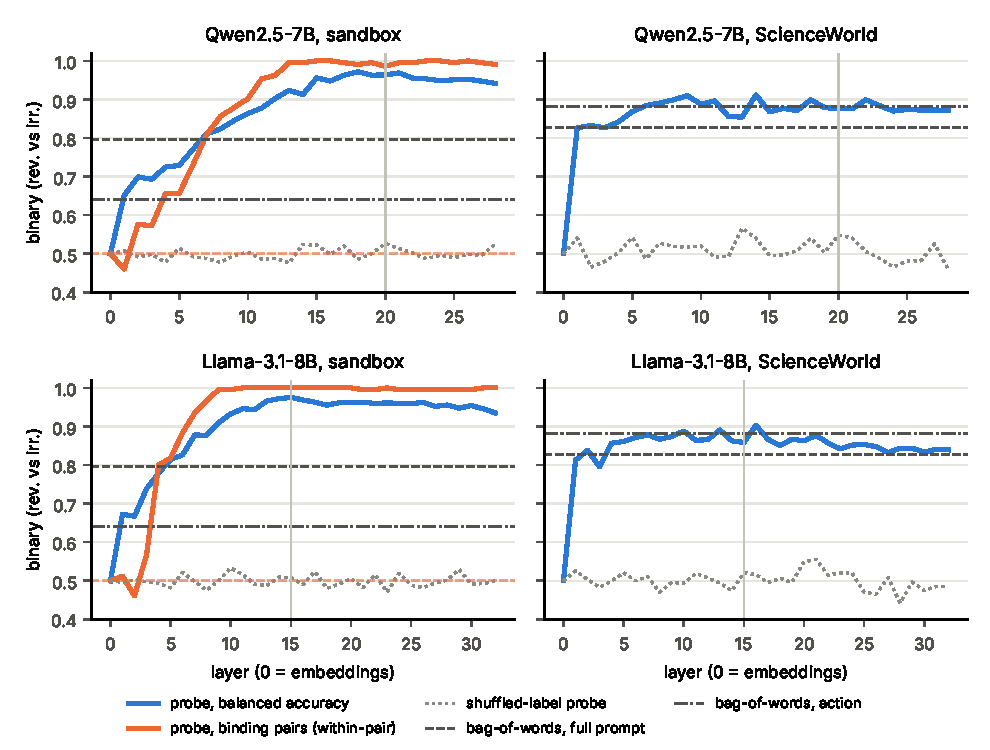
\includegraphics[width=\columnwidth]{fig_probes}
\caption{Binary probes per layer (mean over three scenario splits) with baselines. Orange: within-pair accuracy on binding pairs (identical state text; bag-of-words on the full prompt scores exactly 0.5, thin dashed orange line). Vertical line: the preregistered layer $L^\ast$.}
\label{fig:probes}
\end{figure}

\paragraph{Sandbox: reversibility is linearly decodable, including where text is not enough.} For Qwen, $L^\ast=20$ (chosen on training data). There the binary probe reaches a balanced accuracy of $0.964\pm0.013$ (mean $\pm$ s.d.\ over three splits of $n=344$ test items each; split 0: 0.963 [0.92, 0.99]; AUROC $0.971$), the 3-class probe $0.966\pm0.014$, against $0.80$ for bag-of-words on the full prompt, $0.64$ on the action alone, $0.60$ for the mean-pooled embedding layer, and $0.53$ for a probe trained on shuffled labels (Figure~\ref{fig:probes}). On binding pairs, where the state text is identical and only the action's target differs, the probe ranks the less reversible member higher in $0.986\pm0.011$ of pairs, while every bag-of-words baseline is at exactly $0.5$ by construction. Accuracy rises through the first half of the network and plateaus from about layer 13. Llama behaves the same way with $L^\ast=15$: binary $0.975\pm0.002$ (split 0: 0.977 [0.95, 1.00]; AUROC $0.997$; embedding layer 0.63), 3-class $0.968\pm0.007$, shuffled labels $0.51$, and $1.000$ on binding pairs (plateau from about layer 9).

\paragraph{The control task does not discriminate here.} The control task of \citet{hewitt2019controltasks} (a random fixed label per verb) is solved almost perfectly from layer 1 on ($0.94$ at layer 1, $1.00$ from layer 4), so selectivity is about zero ($-0.04$ at $L^\ast$ for Qwen, $-0.03$ for Llama): with 14 distinct verbs a linear probe can memorise any verb-to-label map. This control therefore says little about our probes; the binding pairs, on which a verb or keyword shortcut is impossible, are the relevant control.

\paragraph{ScienceWorld: no advantage over the surface form.} On 626 ScienceWorld items the probe reaches $0.877\pm0.022$ at $L^\ast$ for Qwen (best layer 14: $0.912$; AUROC $0.975$) and $0.858\pm0.021$ for Llama (best layer 16: $0.903$; AUROC $0.974$), but bag-of-words on the action alone reaches $0.883$: in this environment reversibility is largely predictable from the action text, and our data contain no binding pairs there, so these items cannot separate encoding of the state from encoding of the action.

\paragraph{No transfer between environments.} A probe trained on the sandbox and tested on ScienceWorld at $L^\ast$ reaches a balanced accuracy of $0.58$ (AUROC $0.62$) for Qwen and $0.48$ (AUROC $0.50$) for Llama; in the other direction $0.51$ (AUROC $0.56$) and $0.46$ (AUROC $0.50$). The best single layers reach AUROCs of at most $0.67$. Whatever the sandbox probe reads out is specific to the sandbox's descriptions of bins, backups, undo windows and cancellation windows rather than a general notion of reversibility.

\paragraph{Exploratory: held-out tool domain and within-verb ScienceWorld.} Trained on two of the three sandbox tool domains (files, email, money) and tested on the third, probes at $L^\ast$ fall to balanced accuracies of 0.50--0.64 (Qwen; AUROC 0.59--0.70) and 0.51--0.57 (Llama; AUROC 0.49--0.57), close to bag-of-words on the full prompt (0.51--0.61); on binding pairs they reach 0.51--0.96 and 0.57--0.77. The representation therefore does not carry over to an unseen tool domain either: with 30 contexts that share the same recipes, the sandbox probe can rely on recipe-specific cues, so its near-perfect in-domain accuracy should not be read as a general concept of reversibility. On ScienceWorld, restricted to verbs that occur with both labels in a test split (176 items, pooled over the three splits), the probe ranks irreversible above reversible actions better than bag-of-words on the action (AUROC 0.86 for Qwen and 0.79 for Llama vs.\ 0.69), but at the default threshold its balanced accuracy is not higher (0.61 and 0.58 vs.\ 0.62); with few irreversible items per verb we read this as weak evidence of information beyond the verb.

\paragraph{Encoded vs.\ stated.} On the 312 sandbox items in the seed-0 test split that also have stated answers (Table~\ref{tab:levels}), the 3-class probe at $L^\ast$ is right on 97\% (Cohen's $\kappa=0.96$ with the truth), the stated answer on 45\% ($\kappa=0.17$), and the two agree barely beyond chance ($\kappa=0.15$). In 170 of the 312 items the probe is right and the stated answer wrong; the reverse happens in 6. For Llama the gap is larger: probe 98\% ($\kappa=0.97$), stated 29\% ($\kappa=0.02$, mostly ``partial''), agreement $\kappa=0.02$; probe right and stated wrong in 218 items, the reverse in 2.

\subsection{RQ4: steering}
\begin{figure}[t]
\centering
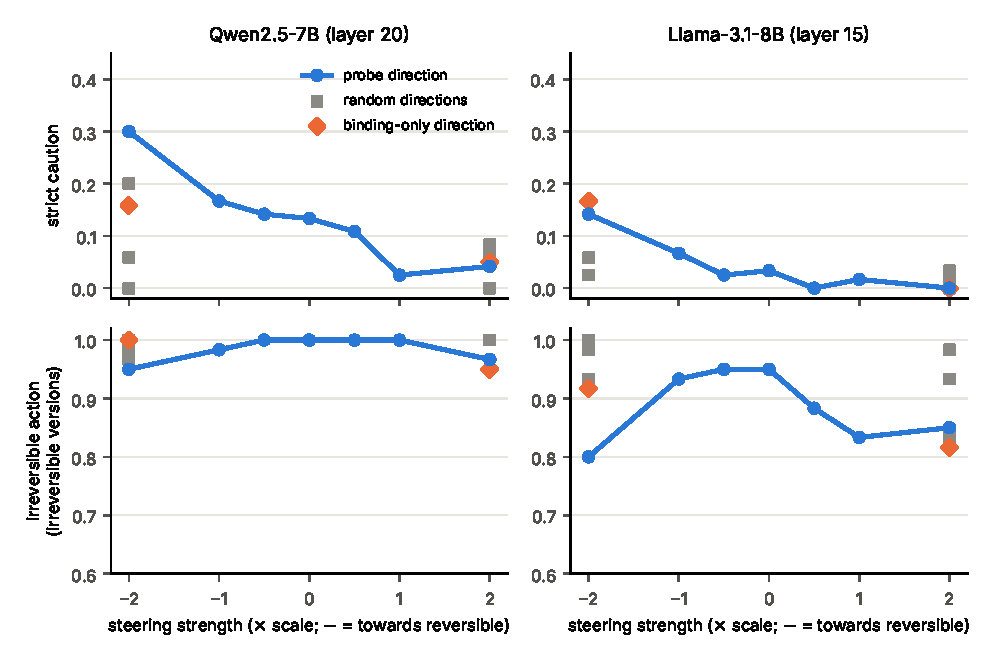
\includegraphics[width=\columnwidth]{fig_steering}
\caption{Steering at $L^\ast$. Top: strict caution (mean of both task versions, 120 episodes per point). Bottom: share of irreversible versions in which the agent took the irreversible action. Strength 0 is the unsteered run; grey squares are three random directions, orange diamonds the direction computed on binding pairs only, both at $\pm2\times$ scale.}
\label{fig:steering}
\end{figure}

Calibration gave the same scale for both models (largest strength with $<$20\% unparseable replies $=0.4\times$ the mean residual norm; at $0.8$ parse failures reached 63\% for Qwen and 29--31\% for Llama), so the test strengths are $\pm0.1, \pm0.2, \pm0.4$. Figure~\ref{fig:steering} shows the results.

\paragraph{Caution moves with the direction, in the unexpected sign.} Pushing activations towards the \emph{reversible} side raises strict caution and pushing towards the \emph{irreversible} side lowers it, in both models. The preregistered logistic regression of strict caution on strength (seven strengths, both versions, 840 episodes) gives slopes of $-0.62$ per unit of scale for Qwen ($p<10^{-9}$; pair-cluster bootstrap 95\% CI $[-0.89,-0.43]$) and $-1.04$ for Llama ($p<10^{-7}$; $[-1.70,-0.63]$).

\paragraph{Specificity differs between the models.} For the difference in strict caution between $-2\times$ and $+2\times$, the probe direction gives $+0.26$ $[0.15, 0.37]$ for Qwen, but one of three random directions gives a similar $+0.20$ $[0.12, 0.28]$ (the others $-0.01$ and $-0.08$), so for Qwen the effect is not specific to the probe direction; most of this change is in \texttt{ask\_user} calls. One component is specific: at $-2\times$ Qwen backs up the file before the shortcut in 15\% of episodes, which never happens unsteered or under any random direction. For Llama the probe direction gives $+0.14$ $[0.08, 0.21]$ against $-0.01$ to $+0.04$ for the random directions; the binding-only direction (cosine with the main direction 0.88 for Qwen, 0.84 for Llama) behaves like the main one ($+0.11$ and $+0.17$).

\paragraph{Exploratory: is it a ``danger'' direction?} A harmful-vs-harmless direction computed as in \citet{arditi2024refusal} (128 AdvBench vs.\ 128 Alpaca requests, last token at $L^\ast$) is nearly orthogonal to the reversibility direction (cosine 0.04 for Qwen, 0.01 for Llama) and separates reversible from irreversible items poorly (AUROC 0.61 and 0.50), although the reversibility direction does separate harmful from harmless requests (AUROC 0.94 and 0.72). Steering along the harm direction at the same strength acts differently: pushing Qwen towards the harmful side makes it decline the shortcut in 20\% of episodes in \emph{both} versions (and 28\% of reversible-version episodes end in unparseable replies), the opposite sign to the reversibility direction, whose irreversible side lowers caution; Llama hardly reacts (caution at most 0.02). The caution shifts in Figure~\ref{fig:steering} are therefore not a generic harm or refusal effect.

\paragraph{The decision itself does not move.} In irreversible versions the agent takes the irreversible action at every strength (Qwen 0.95--1.00; Llama 0.80--0.95, within the range of the random directions, 0.83--1.00), with no trend in either model ($p=0.32$ and $p=0.80$). Confirmation questions stay essentially absent: none along the main or random directions, and 2 (Qwen) and 1 (Llama) of 120 episodes along the binding-only direction at $-2\times$. The cost of steering is small at these strengths: task success stays at 0.86--0.98 (Qwen) and 0.82--0.92 (Llama). In reversible versions, Qwen takes more irreversible actions at both extremes (0.28 at $-2\times$, 0.20 at $+2\times$, 0 unsteered), while Llama takes fewer when pushed towards the irreversible side (0.10 at $+2\times$ vs.\ 0.33 unsteered). The direction that separates reversible from irreversible items therefore changes how much the agent prepares or asks, but it does not make the agent avoid the irreversible step. Because random directions were run only at $\pm2\times$, we cannot test whether they show a trend across strengths; we therefore read RQ4 as weak causal evidence for Llama and no specific evidence for Qwen. Parse failures per strength are listed in \texttt{results/supplement.json}; along the probe direction they stay at or below 1\% of steps for Llama and reach at most 9\% for Qwen (at $+2\times$), below the 20\% calibration limit.

\subsection{Ablations}
\begin{table*}[t]
\centering\small
\resizebox{\linewidth}{!}{%
\begin{tabular}{lcccc}
\toprule
 & \multicolumn{2}{c}{\qwen{} ($L^\ast=20$)} & \multicolumn{2}{c}{\llama{} ($L^\ast=15$)} \\
\cmidrule(lr){2-3}\cmidrule(lr){4-5}
Sandbox probe at $L^\ast$ & mean $\pm$ s.d. & split 0 [95\% CI] & mean $\pm$ s.d. & split 0 [95\% CI] \\
\midrule
Main: binary, last action token & 0.964 $\pm$ 0.013 & 0.963 [0.92, 0.99] & 0.975 $\pm$ 0.002 & 0.977 [0.95, 1.00] \\
(1) Mean over action tokens & 0.970 $\pm$ 0.005 & 0.968 [0.95, 0.99] & 0.980 $\pm$ 0.004 & 0.986 [0.98, 0.99] \\
(2) Train on minimal pairs only & 0.881 $\pm$ 0.005 & 0.878 [0.84, 0.91] & 0.886 $\pm$ 0.007 & 0.895 [0.87, 0.92] \\
(4) Horizon 1 labels$^\dagger$ & 0.940 (1 split) & 0.940 [0.89, 0.98] & 0.961 (1 split) & 0.961 [0.94, 0.98] \\
(4) Horizon 2 labels$^\dagger$ & 0.963 (1 split) & 0.963 [0.93, 0.99] & 0.977 (1 split) & 0.977 [0.95, 1.00] \\
(7) Three classes & 0.966 $\pm$ 0.014 & 0.961 [0.91, 1.00] & 0.968 $\pm$ 0.007 & 0.975 [0.95, 1.00] \\
Layer 0, last token$^\ddagger$ & 0.500 $\pm$ 0.000 & 0.500 [0.50, 0.50] & 0.500 $\pm$ 0.000 & 0.500 [0.50, 0.50] \\
Layer 0, mean over action tokens & 0.600 $\pm$ 0.007 & 0.594 [0.55, 0.63] & 0.626 $\pm$ 0.009 & 0.622 [0.58, 0.67] \\
\midrule
(3) Transfer sandbox $\rightarrow$ ScienceWorld & AUROC 0.62 & 0.583 [0.53, 0.63] & AUROC 0.50 & 0.484 [0.47, 0.49] \\
(3) Transfer ScienceWorld $\rightarrow$ sandbox & AUROC 0.56 & 0.511 [0.50, 0.52] & AUROC 0.50 & 0.463 [0.45, 0.47] \\
(5) Careful prompt: irreversible action, irr.\ versions & 1.00 $\rightarrow$ 1.00 & success 0.98 $\rightarrow$ 0.98 & 0.95 $\rightarrow$ 0.85 & success 0.92 $\rightarrow$ 0.82 \\
\bottomrule
\end{tabular}}
\caption{Ablations. Probe rows: balanced accuracy (binary unless noted) at $L^\ast$, mean $\pm$ s.d.\ over three scenario splits, and the split-0 value with its 95\% scenario-bootstrap CI (test $n=344$ items per split, six held-out contexts). Transfer rows: train on all of one environment, test on all of the other ($n=607$ and $1714$). $^\dagger$One split only (a deviation; see Table~\ref{tab:deviations}). $^\ddagger$The last action token is always the same closing bracket, so this probe is at chance by construction; the mean-pooled layer-0 row is the informative embedding baseline. Ablation (5): irreversible-action rate and task success on the 60 irreversible versions, neutral $\rightarrow$ careful system prompt.}
\label{tab:ablations}
\end{table*}

Table~\ref{tab:ablations} collects the ablations. Averaging over the action's tokens instead of the last token changes little (Qwen $0.970\pm0.005$, Llama $0.980\pm0.004$), so the information is not confined to the final token. Training only on items that belong to a minimal pair lowers accuracy on all test items to about 0.88, i.e.\ unpaired items add useful variety. Transfer between environments is near chance. Only 14 sandbox and 11 ScienceWorld labels change between horizons 1 and 3, so the horizon ablation has little room to differ; it was run on one split only. The 3-class probe is as accurate as the binary one, so partial reversibility is decodable too. The careful system prompt (ablation 5) is discussed under RQ3.

\subsection{Discussion}
The three measurements disagree sharply. In the sandbox, reversibility is linearly decodable from the hidden states almost perfectly, including on binding pairs, where it can only come from combining the action's target with one sentence of the state; the stated answers recover it far less often and the agents not at all. This is the pattern \citet{tang2025riskknowledge} report for risk knowledge and \citet{basu2026actionability} for internal representations more generally: knowing in the representation does not imply using it. Two qualifications keep the claim narrow. The probe's information is environment-specific (no transfer to ScienceWorld or to a held-out tool domain), so we show a sandbox-specific representation of the conditions that make an action undoable, not a general concept of reversibility. And steering along the probe direction changes how much the agent prepares or asks, but never makes it avoid the irreversible step, so we find no evidence that this direction controls the decision. The behavioural findings constrain the interpretation further. Two instruction-tuned models from different families treat a reversible and an irreversible version of the same action identically, even when one sentence of the state decides the difference, and an instruction to be careful does not make them selectively careful. Part of this may be ordinary instruction following: in two task families (send a report, pay an invoice) the irreversible action is itself what the user asked for, and the prompt calls it the fastest option. Their stated judgements are dominated by the verb and by the answer format, but their option probabilities still move with the state in most pairs, so reversibility information is present in some form that neither the final answer nor the behaviour uses.

\section{Limitations}
\textbf{Synthetic sandbox.} Thirty contexts vary surface form, not recipe structure; the sandbox tests controlled distinctions, not the variety of real systems. Labels are relative to our definitions (horizon 3, the tool set, ``partial'' via soft fields or visible content); the models reject the visible-content notion of partial reversibility. \textbf{ScienceWorld labels} come from a pruned search with a node budget; irreversible labels are an upper bound: 51 of the 84 irreversible and 15 of the 16 partial labels hit the search budget, and human agreement on ScienceWorld items is weak ($\kappa=0.44$--$0.66$ with the automatic labels). A re-search of the 66 budget-capped non-reversible items with a five-times larger budget changed 5 labels (7.6\%), all towards reversible (2 irreversible, 3 partial); 57 items still hit the larger budget. With the 2 corrected binary labels the ScienceWorld probe accuracy at L* moves from 0.877 to 0.887 (Qwen) and 0.859 to 0.869 (Llama); conclusions are unchanged, and the main analysis keeps the preregistered labels. The ScienceWorld set is imbalanced (84\% reversible) and has no minimal pairs; stated answers (RQ2) were collected only for the 1,560 main sandbox items, not for ScienceWorld. \textbf{Agent tasks} have a design asymmetry in one family (above), a fixed simulated user, and one scripted shortcut per task; in two families the shortcut is the requested action itself, and strict caution also counts questions that only ask for missing information (all of Qwen's questions). \textbf{Compute}: experiments ran on Kaggle T4 GPUs in fp16 rather than the course GPUs, and the 14B size ablation was not run. \textbf{Statistics}: scenario-clustered intervals rest on six held-out contexts (three held-out tasks for ScienceWorld). The horizon ablation was run on one split rather than three.

\section{Conclusion}
We measured one property, the reversibility of an action, at three levels on shared items for two open-weight model families. In our sandbox it is linearly decodable from the hidden states almost perfectly, including on binding pairs whose text alone cannot decide it, but this representation is specific to the environment and tool domain. The models' stated answers recover it only weakly, and their behaviour as agents does not depend on it at all: they take the irreversible shortcut whether or not it can be undone, and a caution instruction makes them generally, not selectively, more hesitant. Steering along the probe direction changes how much the agent prepares or asks, specifically for Llama, but never stops the irreversible step. Knowing in the representation is therefore far from acting on it, and closing this gap will need more than reading the representation out.

\section*{Ethics Statement}
All actions run in a simulation; no real files, accounts, messages or money are involved. The work aims to make agent failures around irreversible actions measurable. We used no paid APIs for any result.

\paragraph{Use of AI assistants.} An AI assistant (Claude, Anthropic) was used to review the code, data and analyses for errors and to help revise this report, the analysis and table scripts, and the documentation. All reported numbers are produced by the code and saved model outputs in the released repository.

\bibliography{refs}

\appendix
\section{Additional Tables}
\label{sec:appendix}
\begin{table*}[t]
\centering\small
\resizebox{\linewidth}{!}{%
\begin{tabular}{llcccc}
\toprule
Model & Prompt & Strict caution irr./rev. & Broad caution irr./rev. & Broad: sensitivity [CI], McNemar $p$ & Parse failures (episodes ended) \\
\midrule
Qwen-7B & neutral & 0.10 / 0.17 & 0.18 / 0.23 & $-$0.05 [$-$0.12, 0.02], 0.375 & 6 (2) \\
Qwen-7B & careful & 0.07 / 0.15 & 0.15 / 0.18 & $-$0.03 [$-$0.13, 0.07], 0.754 & 0 (0) \\
Llama-8B & neutral & 0.02 / 0.05 & 0.47 / 0.43 & 0.03 [0.00, 0.08], 0.500 & 0 (0) \\
Llama-8B & careful & 0.05 / 0.12 & 0.60 / 0.53 & 0.07 [0.02, 0.13], 0.125 & 0 (0) \\
\midrule
\multicolumn{6}{l}{\emph{Paired 2$\times$2 tables of strict caution (careful in irr.\ only / rev.\ only / both / neither)}} \\
Qwen-7B & neutral & \multicolumn{2}{c}{0 / 4 / 6 / 50} & \multicolumn{2}{l}{gap (prereg.) 0.05 [0.00, 0.12]} \\
Qwen-7B & careful & \multicolumn{2}{c}{1 / 6 / 3 / 50} & \multicolumn{2}{l}{gap (prereg.) 0.03 [$-$0.02, 0.10]} \\
Llama-8B & neutral & \multicolumn{2}{c}{0 / 2 / 1 / 57} & \multicolumn{2}{l}{gap (prereg.) 0.03 [0.00, 0.08]} \\
Llama-8B & careful & \multicolumn{2}{c}{0 / 4 / 3 / 53} & \multicolumn{2}{l}{gap (prereg.) 0.03 [0.00, 0.08]} \\
\bottomrule
\end{tabular}}
\caption{Preregistered secondary RQ3 measures. Broad caution adds inspecting the state (read\_file, list\_files, check\_balance) to strict caution. Parse failures: unparseable replies over all 120 episodes (episodes that ended after three consecutive failures); such episodes are kept.}
\label{tab:secondary}
\end{table*}

\begin{table}[t]
\centering\small
\setlength{\tabcolsep}{3pt}
\resizebox{\linewidth}{!}{%
\begin{tabular}{lccc}
\toprule
Cohen's $\kappa$ [95\% CI] & All ($n=100$) & Sandbox (60) & ScienceWorld (40) \\
\midrule
Annotator A vs.\ B & 0.88 [0.79, 0.96] & 1.00 [1.00, 1.00] & 0.46 [0.06, 0.75] \\
A vs.\ automatic & 0.83 [0.72, 0.93] & 0.95 [0.87, 1.00] & 0.44 [0.10, 0.73] \\
B vs.\ automatic & 0.90 [0.81, 0.97] & 0.95 [0.87, 1.00] & 0.66 [0.27, 0.93] \\
\bottomrule
\end{tabular}}
\caption{Agreement on the blind 100-item sample (three classes; item bootstrap, 1{,}000 resamples).}
\label{tab:kappa}
\end{table}


\section{Deviations from the Preregistration}
\label{sec:deviations}
\begin{table*}[t]
\centering\small
\begin{tabular}{p{0.42\textwidth}p{0.5\textwidth}}
\toprule
Deviation & Reason / effect \\
\midrule
716 extra binding items added to the probe data (2{,}276 instead of 1{,}560) & committed 3\,h after the preregistration, before any hidden state or result existed; more binding pairs for the primary metric \\
Steering direction on all training items (binding-only is a control) & the project brief defines it this way; binding-only direction reported, cosine 0.88/0.84 \\
Random directions at $\pm2\times$ only & allowed by the preregistration if compute is short \\
Probes fitted in the span of the training vectors; Newton solver for binary probes & speed (Kaggle CPU); same objective and solution; a layer with identical vectors gets a chance-level probe \\
RQ2 question limited to the environment's actions; informative simulated user & found in the GPU check and dev pilot, before any stated or test result \\
Kaggle T4 GPUs (fp16) instead of course GPUs & no course GPUs available \\
Horizon ablation (4) on one split instead of three & compute; to be completed \\
\midrule
\multicolumn{2}{p{0.94\textwidth}}{\emph{Exploratory, not preregistered:} probability-based $K$; caution without the safer tool;} \\
\multicolumn{2}{p{0.94\textwidth}}{pair-cluster bootstrap of the steering slope; risk-direction control; held-out tool domain;} \\
\multicolumn{2}{p{0.94\textwidth}}{within-verb ScienceWorld analysis; ScienceWorld label re-search with a larger budget.} \\
\bottomrule
\end{tabular}
\caption{Deviations from the preregistered plan and analyses added afterwards.}
\label{tab:deviations}
\end{table*}
All preregistered analyses are reported, the secondary RQ3 measures in Table~\ref{tab:secondary}. Table~\ref{tab:deviations} lists every change and every analysis added afterwards; exploratory results are labelled as such in the text.

\end{document}
